구간법은 미리 정의된 하한치(lower bound)와 상한치(upper bound)의 경계값으로 이루어지는 구간 내에서 근을 찾았다. 반면에 이장에서 다룰 개구간법(open methods)은 한 개의 초기값에서 시작하거나 구간 내에 근을 포함하지 않을 수도 있는 두 개의 초기값들로부터 시작하는 방법들이다. 이러한 개구간법은 종종 발산(diverge)하거나 근에서 멀어지기도 한다. 그러나 수렴(convergent)할 경우 빠르게 수렴한다.

\subsection{고정점 반복법(fixed point iteration)}
함수 $f(x)=0$의 형태를 다음 식과 같이 변형할 수 있다.
\begin{equation}\label{eq:6-1}
g(x)=x
\end{equation}
이 변형된 함수는 함수 $g$에 대한 \textsl{fixed point}의 해가 된다. 이러한 함수 $f(x)=0$에서 단순한 해법으로 재구성하는 방법은 고정점 반복(fixed point iteration)으로 이루어진다. 그러나 이러한 방법을 수행하기 이전에 우리는 변형된 함수 $g(x)=x$의 해의 존재와 유일성을 검토해야한다. 다음 정리가 이러한 질문에 대한 해를 제시한다.
\begin{theorem}[Fixed-Point Iteration]\label{theo:6-1}
함수 $g(x)$가 구간 $[a,b]$에서 연속의 함수일 때, $\forall x \in [a,b]$에 대해 $g(x)\in [a,b]$ 이면, $g$는 $[a,b]$에서 고정점(fixed point)를 갖는다. 또한, 함수 $g(x)$가 미분가능한 함수이고 아래의 식(\ref{eq:theo-1})과 같은 상수 $k<1$가 존재한다면,
\begin{equation}\label{eq:theo-1}
\left|g'(x)\right|\leq k, x \in (a,b)
\end{equation}
$g$는 정확하게 $[a,b]$에서 하나의 고정점(fixed point)를 갖는다.
\end{theorem}
구간 $[a,b]$에서 고정점을 갖는 연속함수 $g$가 주어진다면, 그 고정점(fixed point)은 구간 $[a,b]$에서 $g(x)=x$를 만족하는 $x$를 무수히 반복하여 찾을 수 있다.

\begin{algorithm}
Let $g$ be a continuous function defined on the interval $[a,b]$. The following algorithm computes a number $x_{r} \in (a,b)$ that is a solution to the equation $g(x)=x$.\\
Choose an initial guess $x_{0}$ in $[a,b]$.

\begin{algorithmic}
\For{$i=0,1,2,\cdots$}
\State $x_{i+1}=g(x_{i})$
\If{$\left|x_{i+1}-x_{i}\right|$ is sufficiently small}
\State $x_{r}=x_{i+1}$
\State \Return $x_{r}$
\EndIf
\EndFor
\end{algorithmic}
\caption{Fixed-Point Iteration}
\end{algorithm}
어떠한 환경에서 고정점 반복이 수렴해서 $x_{r}$을 찾을 수 있을까? 단순히 오차를 $e_{i}=x_{i}-x_{r}$로 가정한다면, Taylor 급수에서 $e_{i+1}\approx g'(x_{r})e_{i}$일 때, $g(x_{r})=x_{r}$임을 찾을 수 있다. 즉, $k<1$일 때, $\left|g'(x_{r})\right| \leq k$ 라면, 고정점 반복(fixed-point iteration)은 부분수렴(locally convergent)한다고 한다. 즉, 초기설정값 $x_{0}$가  $x_{r}$에 충분히 근접한 값을 선택했을 때 수렴한다는 말이다. 이러한 결과는 다음 정리를 통해 알 수 있다.

\begin{theorem}[Fixed-Point Theorem]\label{theo:6-2}
함수 $g(x)$가 구간 $[a,b]$에서 연속의 함수일 때, $\forall x \in [a,b]$에 대해 $g(x)\in [a,b]$ 이고, 다음 식과 같이 상수 $k<1$인 점이 존재한다면,
\begin{equation}\label{eq:theo-2}
\left|g'(x)\right|\leq k, x \in (a,b),
\end{equation}
반복문(the sequence of iterates) $\{x_{i}\}_{i=0}^{\infty}$는 어떤 초기가정 $x_{0} \in [a,b]$에도, 특정 고정값 $x_{r}$으로 수렴하게 된다.
\end{theorem}
함수 $g'(x)$가 수렴의 약조건 $\left|g'(x)\right|<1$에 비하여 $(a,b)$에서 $1$과 떨어지도록 경계지어야하는지에 대하여, 만약 $g'(x)$가 $x$가 어느 한점 $c \in (a,b)$로 접근할 때 $1$로의 접근을 허용한다면, 오차 $e_{i}$가 $i$가 증가할 수록 $0$으로 수렴하지 않을 수가 있다. 이러한 경우 고정점 반복법(fixed-point iteration)은 수렴하지 않는다.

일반적으로 고정점 반복(fixed-point iteration)이 수렴할 때, $\left|g'(x)\right|$의 경계치는 상수 $k$의 역으로 변화하면서 수렴한다.

한편, $f(x)=0$를 $g(x)=x$로 변환하는 식은 많은 방법이 존재하지만, 단순화된 방법으로 특정함수 $\phi(x)$를 추가한 $g(x)=x-\phi(x)f(x)$방법을 사용한다. 그러나 이러한 함수변형에 있어 가장 중요한 요소는 함수 $g(x)$의 수렴성이다.
\begin{figure}[!hbpt]
\centering
\subfigure[$g(x)=\cos(x)$]{
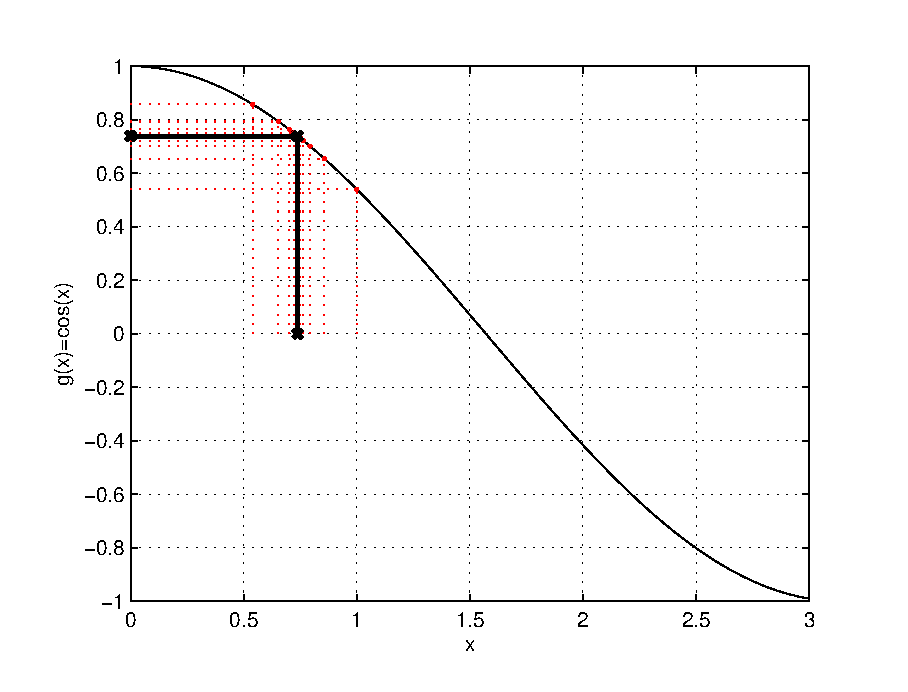
\includegraphics[keepaspectratio=true,width=0.4\linewidth]{figs/fpi-cos.eps}}
\subfigure[$g(x)=\exp(-x)$]{
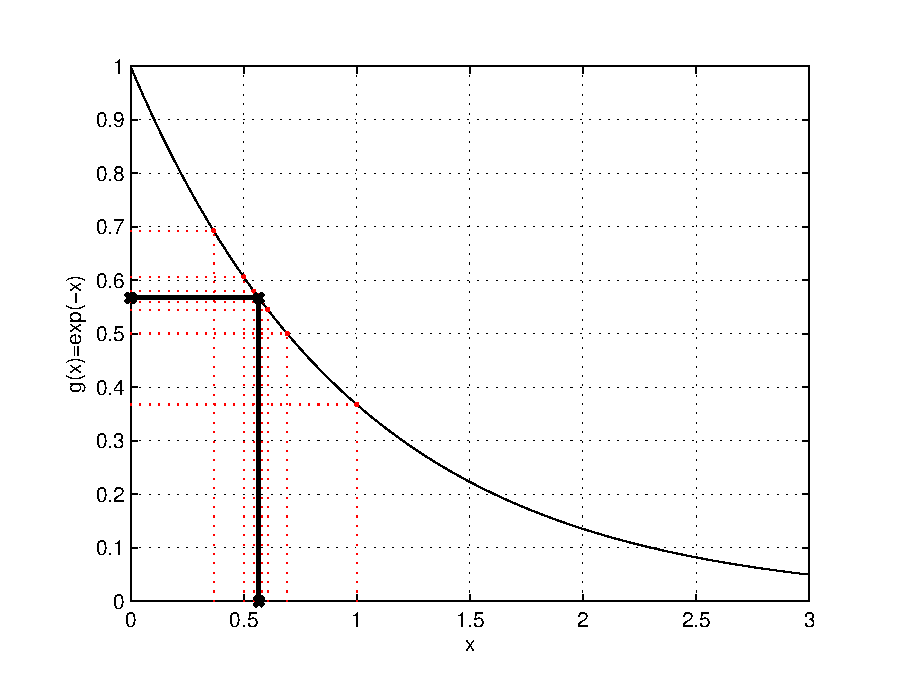
\includegraphics[keepaspectratio=true,width=0.4\linewidth]{figs/fpi-exp.eps}}
\caption{고정점 반복법의 수렴과정}
\label{fig:6-1}
\end{figure}
\clearpage
\subsection{Newton-Raphson법 (Newton-Raphson method)}
구간법의 문제점은 적어도 한 근을 포함하는 구간을 알고있어야 한다는 점이다. 즉, 이러한 방법은 필요한 구간을 상정하기 위해서 무수히 많이 반복을 수행해야하기 때문에 실용적이지 못하다. 좀더 효과적으로 근을 구하는 방법을 찾기 위해서는 다음과 같은 질문을 해결해야 한다.
\begin{itemize}
\item Are there cases in which the problem easy to solve, and if so, how do we solve it in such cases?
\item Is it possible to apply our method of solving the problem in these "easy" cases to more general cases?
\end{itemize}
근을 구하는 공식들 중에서 가장 일반적으로 사용하는 것이 Newton-Raphson 법이다. 근에 대한 초기가정값이 $x_{i}$라면, 점 $[x_{i},f(x_{i})]$에 접하는 접선을 구할 수 있고, 이 접선이 $x$축과 교차하는 점이 개선된 근이 된다.
\ref{ch:4-1}장 \pageref{eq:4-7}페이지 식(\ref{eq:4-7})의 Taylor 급수를 통해 1차항으로 구성된 다음 식으로 근사화 시킬 수 있다.
\begin{equation}
f(x_{i+1})\cong f(x_{i})+f'(x_{i})(x_{i+1}-x_{i})
\end{equation}
즉, $x$축과의 교점에서 $f(x_{i+1})=0$이 되므로 다음과 같이 근사할 수 있다.
\begin{equation}
0=f(x_{i})+f'(x_{i})(x_{i+1}-x_{i})
\end{equation}
$x_{i+1}$에 대하여 정리하면 다음식(\ref{eq:6-6})과 같다.
\begin{equation}\label{eq:6-6}
x_{i+1}=x_{i}-\frac{f(x_{i})}{f'(x_{i})}
\end{equation}

\begin{algorithm}
Let $f:\mathbb{R}\rightarrow\mathbb{R}$ be a differentiable function. The following algorithm computes an approximate solution $x_{r}$ to the equation $f(x)=0$.\\
Choose an initial guess $x_{0}$.
\begin{algorithmic}
\For{$i=0,1,2,\cdots$}
  \If{$f(x_{i})$ is sufficiently small}
    \State $x_{r}=x_{i}$
    \State \Return $x_{r}$
  \EndIf
  \State $x_{i+1}=x_{i}-\frac{f(x_{i})}{f'(x_{i})}$
  \If{$\left|x_{i+1}-x_{i}\right|$ is sufficiently small}
    \State $x_{r}=x_{i+1}$
    \State \Return $x_{r}$
  \EndIf
\EndFor
\end{algorithmic}
\caption{Newton-Raphson Method}
\end{algorithm}
Newton-Raphson법이 수렴할때, 상당히 빨리 수렴한다. 그러나, 수렴 여부에 대해 찾기가 쉽지 않을 수 있다. 특히, 함수 $f(x)$가 근의 부근 $x_{r}$에서 수평기울기(horizontal tangent)을 가지게 될 때 반복구간에서 값이 커질 수가 있다. 이러한 경우 일반적으로 시작지점 $x_{0}$을 $x_{r}$에 가장 가까운 곳에서 선택할 필요가 있다.
\begin{theorem}[Convergence of Newton-Raphson's Method]
함수 $f(x)$를 구간 $[a,b]$에서 연속이며 미분가능하다고 가정하고, 특정한 값 $c \in [a,b]$에서 $f(c)=0$와 $f'(c)=0$을 만족한다고 가정하면, 함수 $f(x)$에 Newton-Raphson법을 적용했을때 $[c-\delta,c+\delta]$구간에서 수렴하는 어떤 초기값 $x_{0}$을 갖는 $\delta >0$인 $\delta$가 존재한다.
\end{theorem}

\framebox{예제} \textbf{Newton-Raphson법 예제 ($\sqrt{2}$ 찾기)}\\
\rule{\textwidth}{0.1pt}
다음 함수 $f(x)$를 통해 $\sqrt{2}$의 값을 Newton-Raphson법을 이용하여 예측하라.
\begin{equation}
f(x)=x^2 -2
\end{equation}
\framebox{해}
$f'(x)=2x$이기 때문에, Newton-Raphson법에서 $x_{i}$에 대한 $x_{i+1}$은 다음식과 같다.
\begin{equation}
x_{i+1}=x_{i}-\frac{f(x_{i})}{f'(x_{i})}
=x_{i}-\frac{x_{i}^2-2}{2x_{i}}
=\frac{x_{i}}{2}+\frac{1}{x_{i}}
\end{equation}

\begin{table}[!hbpt]
\centering
\begin{tabular}{l|l|l|c}
\hline
\hline
\boldmath $x_{i}$ & \boldmath $f(x_{i})$ &\boldmath $f'(x_{i})$ & \textbf{Tangent line}\\
\hline
$x_{0}=0.5 $ & $f(x_{0})=-1.75$ & $f'(x_{0})=1$ & $y=f'(x_{0})(x-x_{0})+f(x_{0})$\\
$x_{1}=2.25 $ & $f(x_{1})=3.0625$ & $f'(x_{1})=4.5$ & $y=f'(x_{1})(x-x_{1})+f(x_{1})$\\
$x_{2}=1.5694 $ &  $f(x_{2})=0.463155$ & $f'(x_{2})=3.13889$ & $y=f'(x_{2})(x-x_{2})+f(x_{2})$\\
$x_{3}=1.42189 $ & $f(x_{3})=2.177221\times10^{-2}$ & $f'(x_{3})=2.84378$ & $y=f'(x_{3})(x-x_{3})+f(x_{3})$\\
$x_{4}=1.414234 $ & $f(x_{4})=5.861552\times10^{-5}$ & $f'(x_{4})=2.82847$ & $y=f'(x_{4})(x-x_{4})+f(x_{4})$\\
\hline
\end{tabular}
\end{table}

\begin{figure}[!hbpt]
\centering
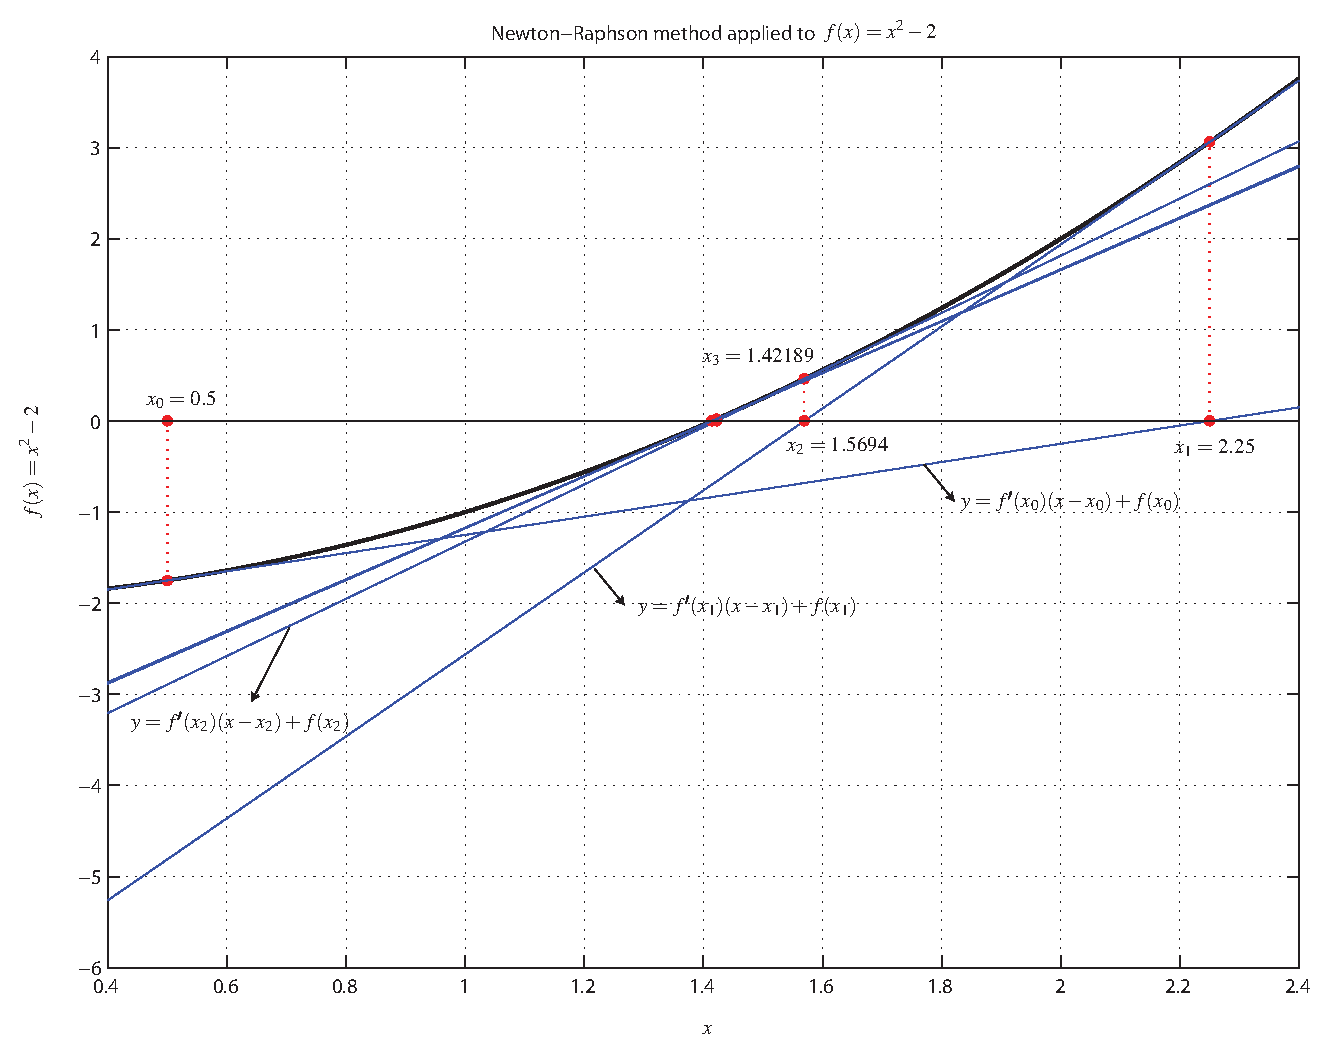
\includegraphics[keepaspectratio=true,width=0.7\textwidth]{figs/newton1.eps}
\caption{Newton-Raphson Method}
\label{fig:6-2}
\end{figure}
\clearpage
\subsection{할선법 (secant method)}
Newton-Raphson법을 수행하는데 어려운점은 바로 도함수의 계산이다. 어떤 함수에서는 도함수를 계산하는 것이 매우 어려울 수 있다. 그러한 경우 도함수는 \ref{sec:4-diff}장에서 학습한 수치미분중 후진유한제차분으로 근사시킬 수 있다. 후진차분근사법은 식(\ref{eq:4-backward})에서 도함수를 가져오기로 하자.
\begin{equation}\label{eq:6-backward}
f'(x_{i})\cong\frac{f(x_{i-1})-f(x_{i})}{x_{i-1}-x_{i}}
\end{equation}
도함수의 후진차분근사 식(\ref{eq:6-backward})을 Newton-Raphson법 식(\ref{eq:6-6})에 대입시킨다.
\begin{equation}\label{eq:6-7}
x_{i+1}=x_{i}-\frac{f(x_{i})(x_{i-1}-x_{i})}{f(x_{i-1})-f(x_{i})}
\end{equation}
식(\ref{eq:6-7})과 같이 할선법(secant method)는 두개의 초기값 $x_{i-1}$, $x_{i}$이 필요하다. 즉, $x_{2}$부터 추적해나가기 때문에 $x_{0}$과 $x_{1}$의 초기값이 필요하다.

\begin{algorithm}
Let $f:\mathbb{R}\rightarrow\mathbb{R}$ be a differentiable function. The following algorithm computes an approximate solution $x_{r}$ to the equation $f(x)=0$.\\
Choose an initial guess $x_{0}$ and $x_{1}$.
\begin{algorithmic}
\For{$i=0,1,2,\cdots$}
  \If{$f(x_{i})$ is sufficiently small}
    \State $x_{r}=x_{i}$
    \State \Return $x_{r}$
  \EndIf
  \State $x_{i+2}=x_{i+1}-\frac{f(x_{i+1})(x_{i}-x_{i+1})}{f(x_{i})-f(x_{i+1})}$
  \If{$\left|x_{i+2}-x_{i+1}\right|$ is sufficiently small}
    \State $x_{r}=x_{i+2}$
    \State \Return $x_{r}$
  \EndIf
\EndFor
\end{algorithmic}
\caption{Secant Method}
\end{algorithm}

\clearpage
\subsection{수정된 할선법 (modified secant method)}
도함수를 계산하기 위하여 임의의 두 값을 사용하기보다 $f'(x)$를 추정하기 위하여 독립변수에 약간의 변동을 주는 방법을 고려할 수 있다.
\begin{equation}
f'(x_{i})\cong \frac{f(x_{i}+\delta x_{i})-f(x_{i})}{\delta x_{i}}
\end{equation}
여기서 $\delta$는 약간의 변동량이다.식(\ref{eq:6-6})에 위의 식을 대입하면 다음과 같은 반복계산식을 얻을 수 있다.
\begin{equation}\label{eq:6-8}
x_{i+1}=x_{i}-\frac{\delta x_{i}f(x_{i})}{f(x_{i}+\delta x_{i})-f(x_{i})}
\end{equation}

\begin{algorithm}
Let $f:\mathbb{R}\rightarrow\mathbb{R}$ be a differentiable function. The following algorithm computes an approximate solution $x_{r}$ to the equation $f(x)=0$.\\
Choose an initial guess $x_{0}$ and $\delta$.
\begin{algorithmic}
\For{$i=0,1,2,\cdots$}
  \If{$f(x_{i})$ is sufficiently small}
    \State $x_{r}=x_{i}$
    \State \Return $x_{r}$
  \EndIf
  \State $x_{i+1}=x_{i}-\frac{\delta x_{i}f(x_{i})}{f(x_{i}+\delta x_{i})-f(x_{i})}$
  \If{$\left|x_{i+1}-x_{i}\right|$ is sufficiently small}
    \State $x_{r}=x_{i+1}$
    \State \Return $x_{r}$
  \EndIf
\EndFor
\end{algorithmic}
\caption{Modified Secant Method}
\end{algorithm}
이 수정된 할선법 알고리즘에서 $\delta$의 선택이 이슈가 되는데 적절하게 $\delta$를 선택하는 방법밖에는 없다. $\delta$가 작으면 식(\ref{eq:6-8})의 분모에서 발생하는 반올림 오차가 커지게되고, 또한 $\delta$가 커지게 되면 발산할 수도 있다. 그러나 적절한 $\delta$가 선택되면 도함수를 계산하기 어려운 함수의 근이나 두개의 초기가정을 결정하는 것이 어려운 경우 근을 찾는 좋은 방법이 될 수 있다.